\documentclass[tikz,border=8pt]{standalone}
\usepackage{tikz}
\usetikzlibrary{positioning,fit,shapes.geometric}

\begin{document}

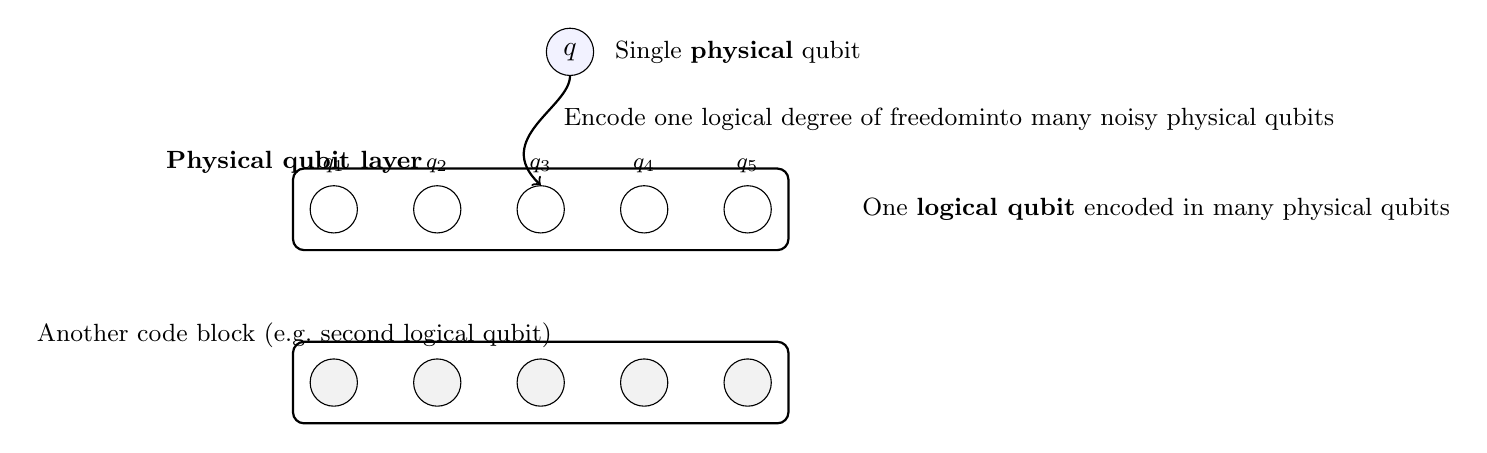
\begin{tikzpicture}[
=latex,
   qubit/.style={circle, draw, minimum size=6mm, inner sep=0pt},
   logical/.style={rounded corners=4pt, draw, thick, inner sep=6pt},
   label/.style={font=\small}
]

% --- Top: single physical qubit -----------------------------
\node[qubit, fill=blue!5] (phys_single) at (0,2) {$q$};
\node[label, right=4pt of phys_single.east] {Single \textbf{physical} qubit};

% --- Middle: many physical qubits forming one logical qubit --
\node[label] at (-3.5,0.6) {\textbf{Physical qubit layer}};

% 5 physical qubits in a row
\node[qubit] (p1) at (-3,0) {};
\node[qubit] (p2) [right=0.7cm of p1] {};
\node[qubit] (p3) [right=0.7cm of p2] {};
\node[qubit] (p4) [right=0.7cm of p3] {};
\node[qubit] (p5) [right=0.7cm of p4] {};

\node[label, above=1pt of p1] {\footnotesize $q_1$};
\node[label, above=1pt of p2] {\footnotesize $q_2$};
\node[label, above=1pt of p3] {\footnotesize $q_3$};
\node[label, above=1pt of p4] {\footnotesize $q_4$};
\node[label, above=1pt of p5] {\footnotesize $q_5$};

% Bracket / fit box for logical qubit
\node[logical, fit=(p1) (p5), label={[label]below:$\lvert 0_L\rangle$}] (logical1) {};

\node[label, right=0.8cm of logical1.east] {One \textbf{logical qubit} encoded in many physical qubits};

% --- Bottom: another logical qubit built from many physical qubits ---
\node[label] at (-3.5,-1.6) {Another code block (e.g.\ second logical qubit)};

\node[qubit, fill=gray!10] (q1b) at (-3,-2.2) {};
\node[qubit, fill=gray!10] (q2b) [right=0.7cm of q1b] {};
\node[qubit, fill=gray!10] (q3b) [right=0.7cm of q2b] {};
\node[qubit, fill=gray!10] (q4b) [right=0.7cm of q3b] {};
\node[qubit, fill=gray!10] (q5b) [right=0.7cm of q4b] {};

\node[logical, fit=(q1b) (q5b), label={[label]below:$\lvert 1_L\rangle$}] (logical2) {};

% --- Legend arrows -------------------------------------------
\draw[->, thick] (phys_single.south) .. controls (0,1.3) and (-1.0,0.9) .. (p3.north)
   node[midway, right, xshift=6pt, yshift=2pt, label]
   {Encode one logical degree of freedom\\into many noisy physical qubits};

\end{tikzpicture}

\end{document}
